%Master File:lectures.tex


\lesson{Symmetry}
\vspace{-1cm}
\begin{center}
  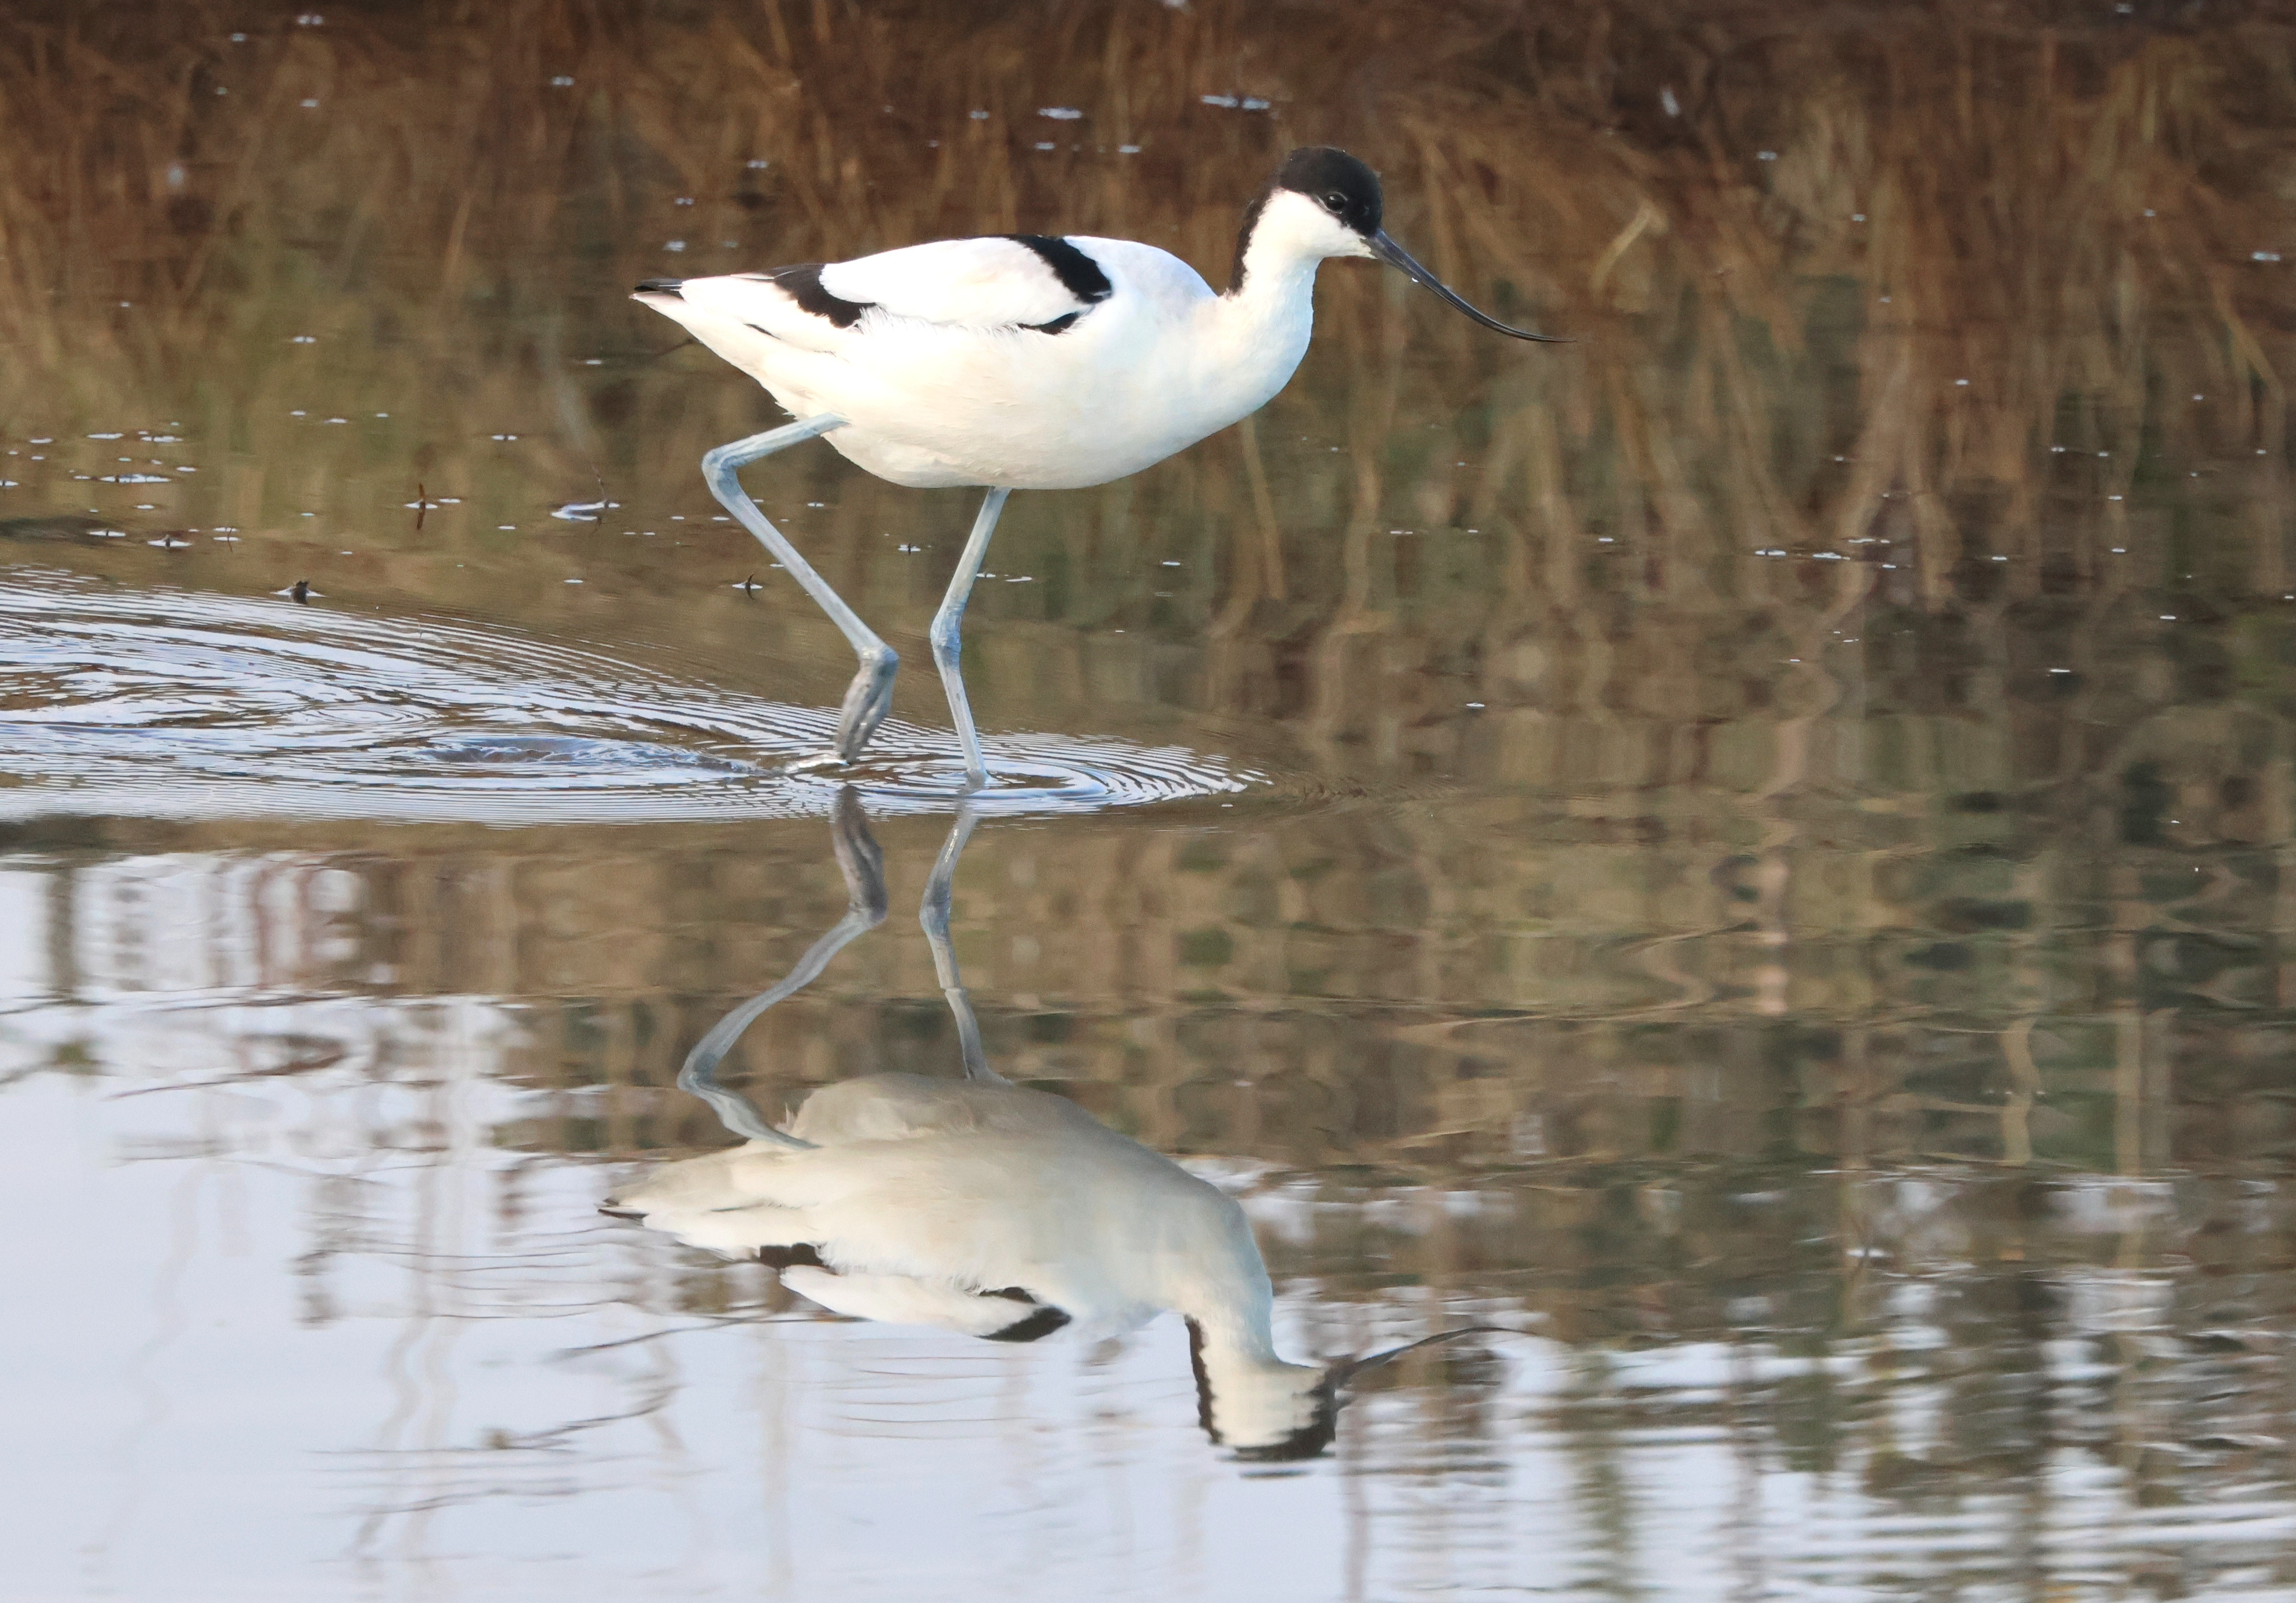
\includegraphics[height=10cm]{symmetry.JPG}
\end{center}
\keywords{Inductive Bias, Symmetry, Invariance, Group theory}
%%%%%%%%%%%%%%%%%%%%%%% Next Slide %%%%%%%%%%%%%%%%%%%%%%%
\renewcommand{\Outline}{%
\begin{slide}
\section[1]{Outline}

\begin{minipage}{10cm}\raggedright
  \begin{enumerate}\squeeze
    \outlineitem{Inductive Bias}{inductivebias}
    \outlineitem{Invariance}{invariance}
    \outlineitem{Group Theory}{grouptheory}
  \end{enumerate}
\end{minipage}\hfill
\begin{minipage}{12cm}
  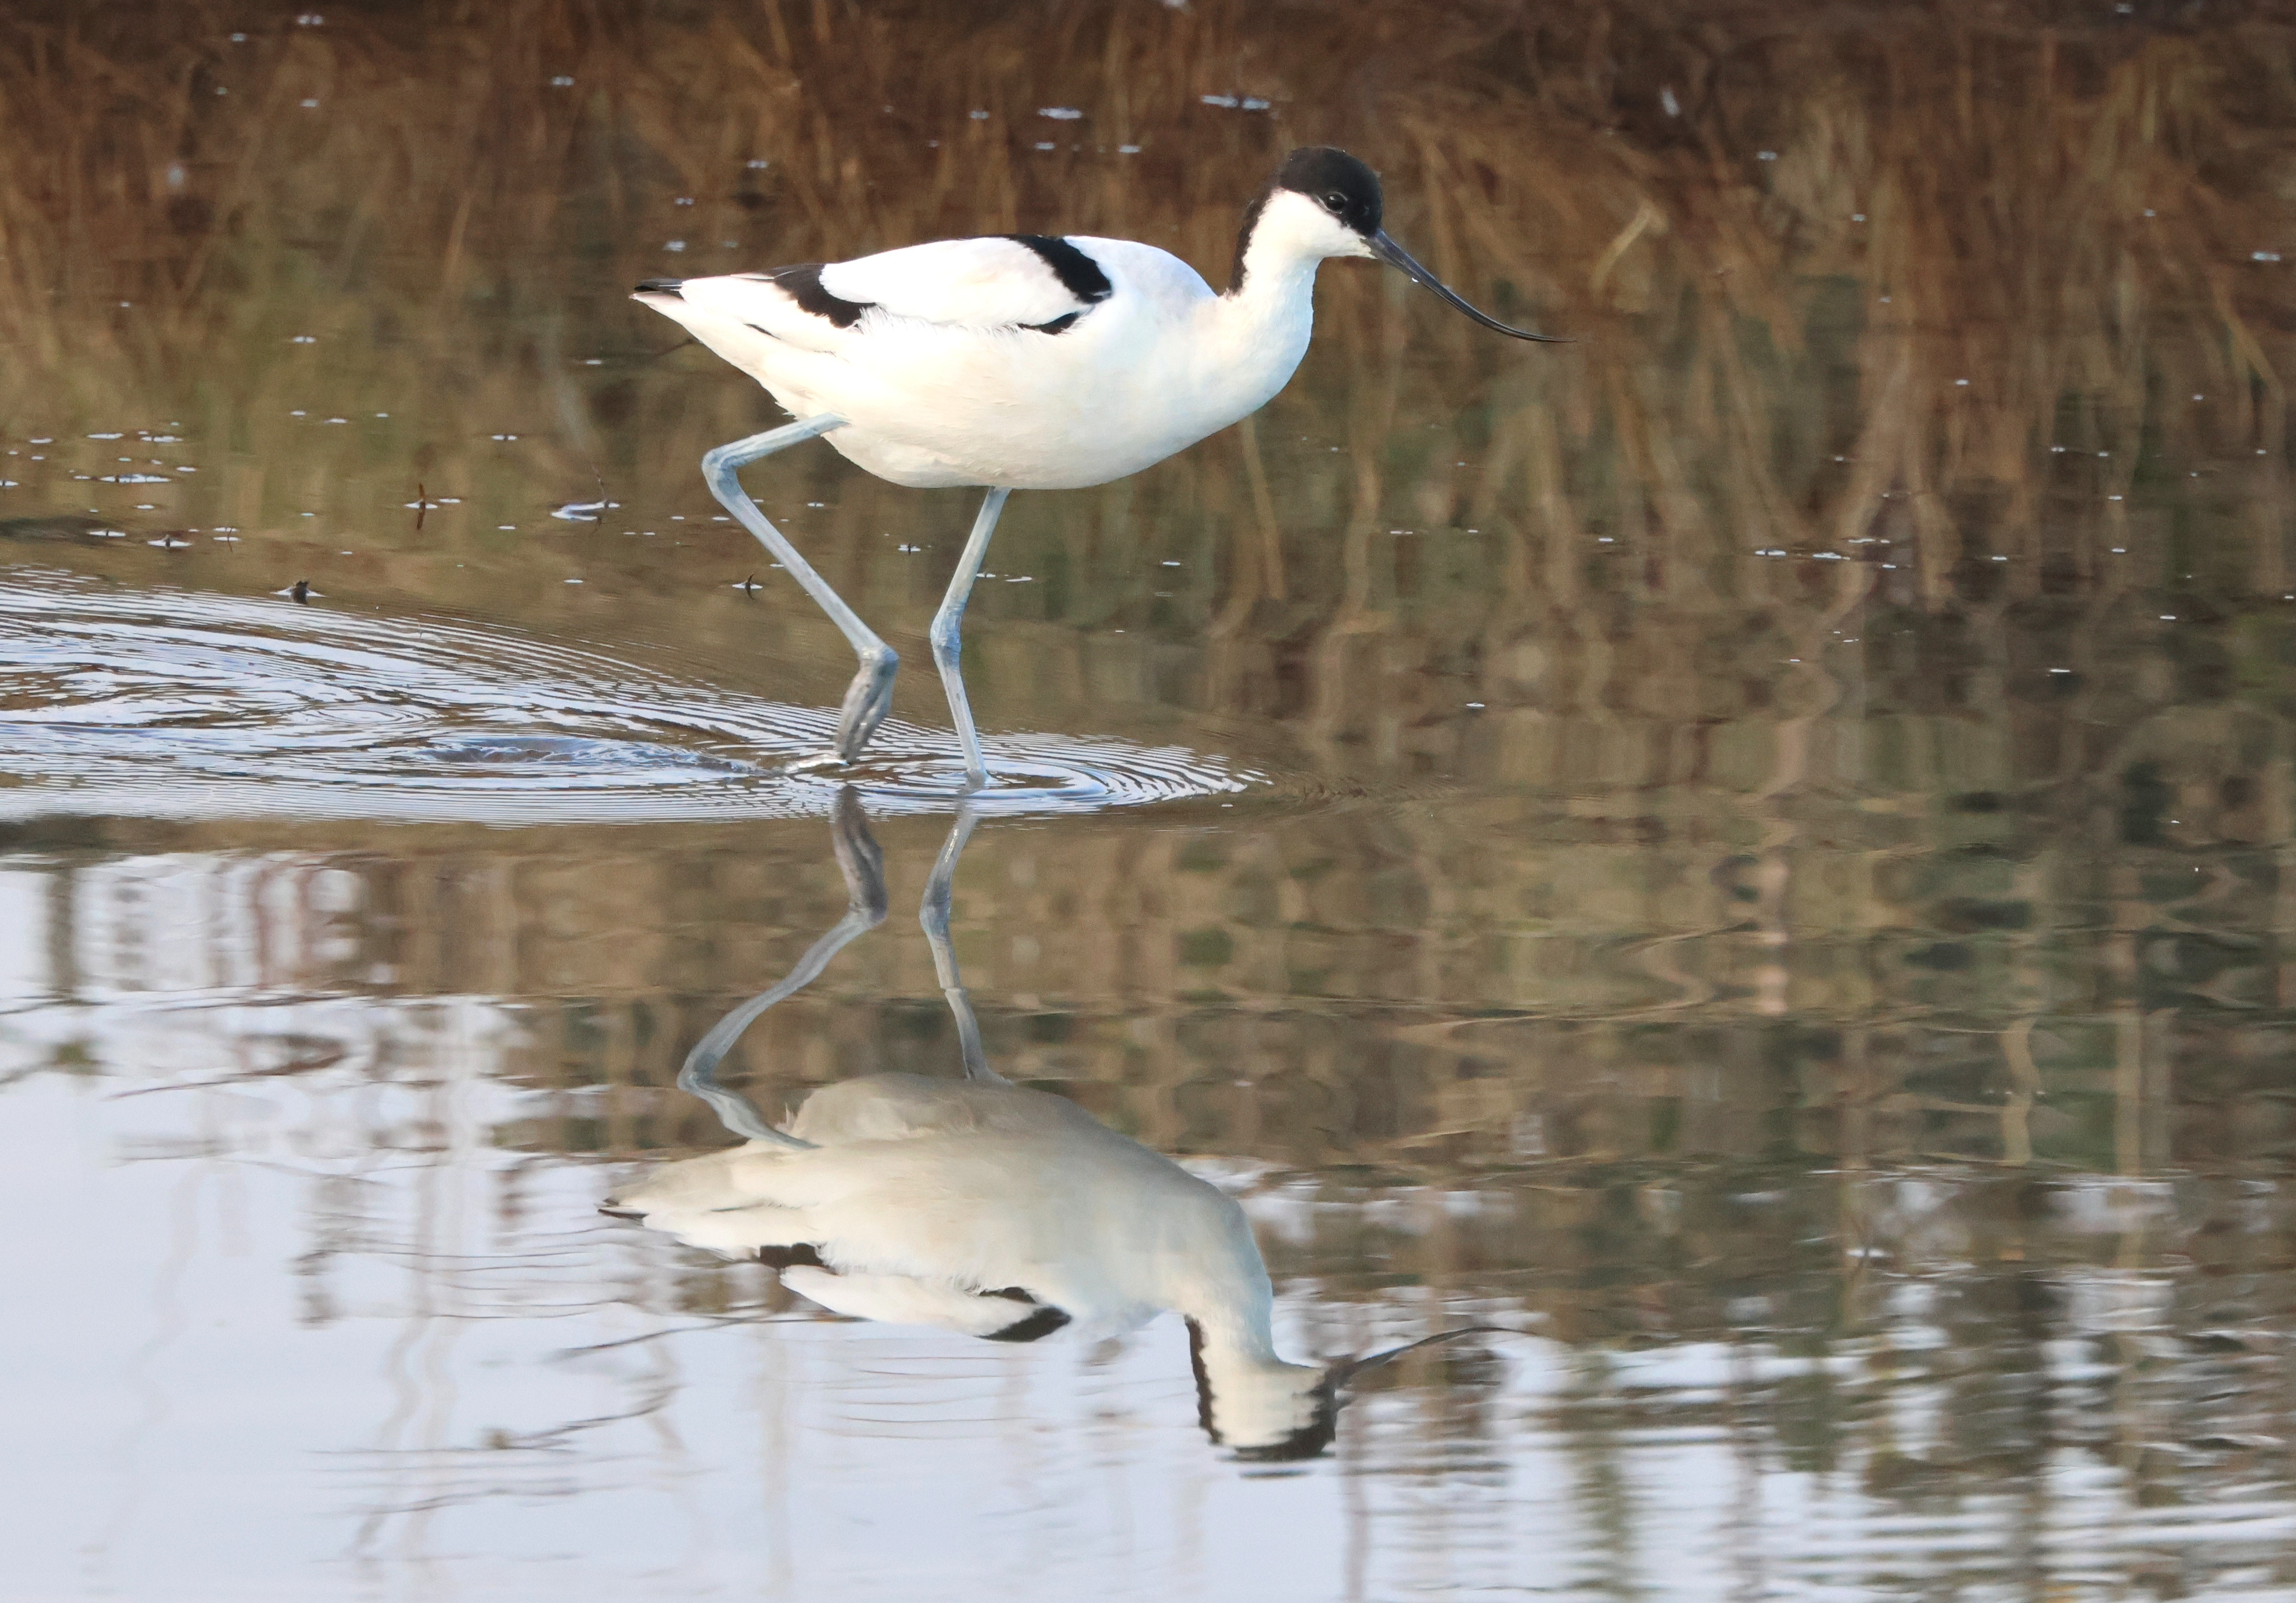
\includegraphics[width=11.5cm]{symmetry.JPG}
\end{minipage}
\end{slide}
\addtocounter{outlineitem}{1}
}

\setcounter{outlineitem}{1}
%%%%%%%%%%%%%%%%%%%%%%% Next Slide %%%%%%%%%%%%%%%%%%%%%%%
\Outline % Introduction
\toptarget{firstoutline}
%%%%%%%%%%%%%%%%%%%%%%% Next Slide %%%%%%%%%%%%%%%%%%%%%%%

\begin{slide}
\section{Inductive Bias}

\begin{PauseHighLight}
  \begin{itemize}
  \item Learning machines differ in how they split up the space of
    inputs\pause
  \item Perceptrons split the space using a hyperplane, RBFs split the space
    depending on some set of centres, MLPs successive split the world
    at different layers\pause
  \item These differences are known as the \emph{inductive bias} of
    the machine\pause
  \item The different inductive bias lead to different
    performance\pause
  \item How can we exploit the inductive bias to get good performance?\pause
  \end{itemize}
\end{PauseHighLight}

\end{slide}

%%%%%%%%%%%%%%%%%%%%%%% Next Slide %%%%%%%%%%%%%%%%%%%%%%%

\begin{slide}
\section{The Real World}

\begin{PauseHighLight}
  \begin{rightImage}{distinctClasses}
  \begin{itemize}
  \item The problems that we care about come from a highly structured
    world  where the solutions inherit some of the properties of that
    world\pause
  \item Usually similar input have similar outputs (we don't expect to
    change one pixel in an image and that it should be classified
    differently)\pause
  \item The classes are often quite well separated\pause
  \end{itemize}
  \end{rightImage}
\end{PauseHighLight}

\end{slide}

%%%%%%%%%%%%%%%%%%%%%%% Next Slide %%%%%%%%%%%%%%%%%%%%%%%

\begin{slide}
\section{Smoothness}

\begin{PauseHighLight}
  \begin{itemize}
  \item A natural assumption is smoothness (the classification surface
    or regression surface changes slowly as we change the input)\pause
  \item Often there is a hyperparameter that controls this
    \begin{itemize}
    \item The kernel parameter $\gamma$ in SVMs (or $\ell$ in Gaussian
      Processes)
    \item $k$ in $k$-nearest neighbours
    \item The size of the $L_2$ regulisation term in neural networks\pause
    \end{itemize}
  \item We often have to choose these using trial and error (using a
    validation set)\pause
  \end{itemize}
\end{PauseHighLight}

\end{slide}

%%%%%%%%%%%%%%%%%%%%%%% Next Slide %%%%%%%%%%%%%%%%%%%%%%%
\Outline % Invariance
%%%%%%%%%%%%%%%%%%%%%%% Next Slide %%%%%%%%%%%%%%%%%%%%%%%

\begin{slide}
\section{Symmetry}
  
\begin{PauseHighLight}
  \begin{itemize}
  \item There are sometimes symmetries in the world we can
    exploit\pause
  \item In image classification we consider an object should be
    classified the same wherever it is in the image\pause
  \item The classification should be invariant to translations
    (scaling and perhaps rotations)\pause
  \item The classification function possesses a translational
    symmetry\pause
  \item Learning machines that respect translational invariance have
    far less propensity to overfit\pause---they don't need to learn
    that the same object in a different part of the image is the same\pauseb
  \end{itemize}
\end{PauseHighLight}

\end{slide}

%%%%%%%%%%%%%%%%%%%%%%% Next Slide %%%%%%%%%%%%%%%%%%%%%%%

\begin{slide}
  \section{Convolutional Neural Networks}

  \pb
\pause \pauselevel{=1}
\begin{center}
  \multipdf[width=\linewidth]{cnnSchematic}\pause
\end{center}
\end{slide}

%%%%%%%%%%%%%%%%%%%%%%% Next Slide %%%%%%%%%%%%%%%%%%%%%%%

\begin{slide}
\section{Equivariance}

\begin{PauseHighLight}
  \begin{itemize}
  \item CNNs are not translationally invariant\pause
  \item The output will be different if we shift the input\pause
  \item They are (up to edge effects) \emph{equivariant} in that we would get
    the same result if we shifted both the input and the output in the
    same way\pause
  \item They are not perfectly equivariant (they break at the pixel
    level and at the full image level---due to edges)\pause
  \item But they are sufficient good that CNNs have dominated computer
    vision for years\pause{} (ignoring visual transformers)\pauseb
  \end{itemize}
\end{PauseHighLight}

\end{slide}

%%%%%%%%%%%%%%%%%%%%%%% Next Slide %%%%%%%%%%%%%%%%%%%%%%%

\begin{slide}
\section{Other Symmetries}

\begin{PauseHighLight}
  \begin{itemize}
  \item The identity of an object should not change if we move the
    camera further away or rotate the camera\pause
  \item CNNs are not naturally scale or rotationally invariant\pause{}
    (although there are attempts to remedy this)\pauseb
  \item Rotation invariance doesn't always reflect ``the
    world''\pause---people usually stand on their feet not on their
    heads\pause
  \item Although you want rotational invariance when interpreting
    aerial images\pause
  \end{itemize}
\end{PauseHighLight}

\end{slide}

%%%%%%%%%%%%%%%%%%%%%%% Next Slide %%%%%%%%%%%%%%%%%%%%%%%

\begin{slide}
\section{Scale Symmetry}

\begin{PauseHighLight}
  \begin{rightImage}[0.35]{Image_pyramid}
  \begin{itemize}
  \item CNNs are not scale invariant\pause
  \item There are various pyramid image processing techniques to try
    and build in approximate scale invariance\pause
  \item However, in many image classification tasks we concentrate on
    the object in the foreground\pauseb
  \item Many datasets rescale objects in the image so
    they are roughly the same size\pauseb
  \end{itemize}
  \end{rightImage}
\end{PauseHighLight}

\end{slide}

%%%%%%%%%%%%%%%%%%%%%%% Next Slide %%%%%%%%%%%%%%%%%%%%%%%

\begin{slide}
\section{Learning Invariance}

\begin{PauseHighLight}
  \begin{itemize}
  \item Currently we are  not smart enough to come up with networks
    that are scale invariant or rotational invariant\pause{} or
    invariant to small distortions\pauseb
  \item We therefore hope that our networks learns this by training on
    objects of different sizes, orientations, lighting conditions,
    etc.\pause
  \item Knowing this is an invariance we want, it is now common
    practice to do data augmentation where we perform transformations
    that replicate physical plausible changes in the data\pause
  \item We are removing spurious rules by (artificially) increasing
    our dataset size\pause
  \end{itemize}
\end{PauseHighLight}

\end{slide}

%%%%%%%%%%%%%%%%%%%%%%% Next Slide %%%%%%%%%%%%%%%%%%%%%%%

\begin{slide}
\section{Augmentations}

\begin{center}
  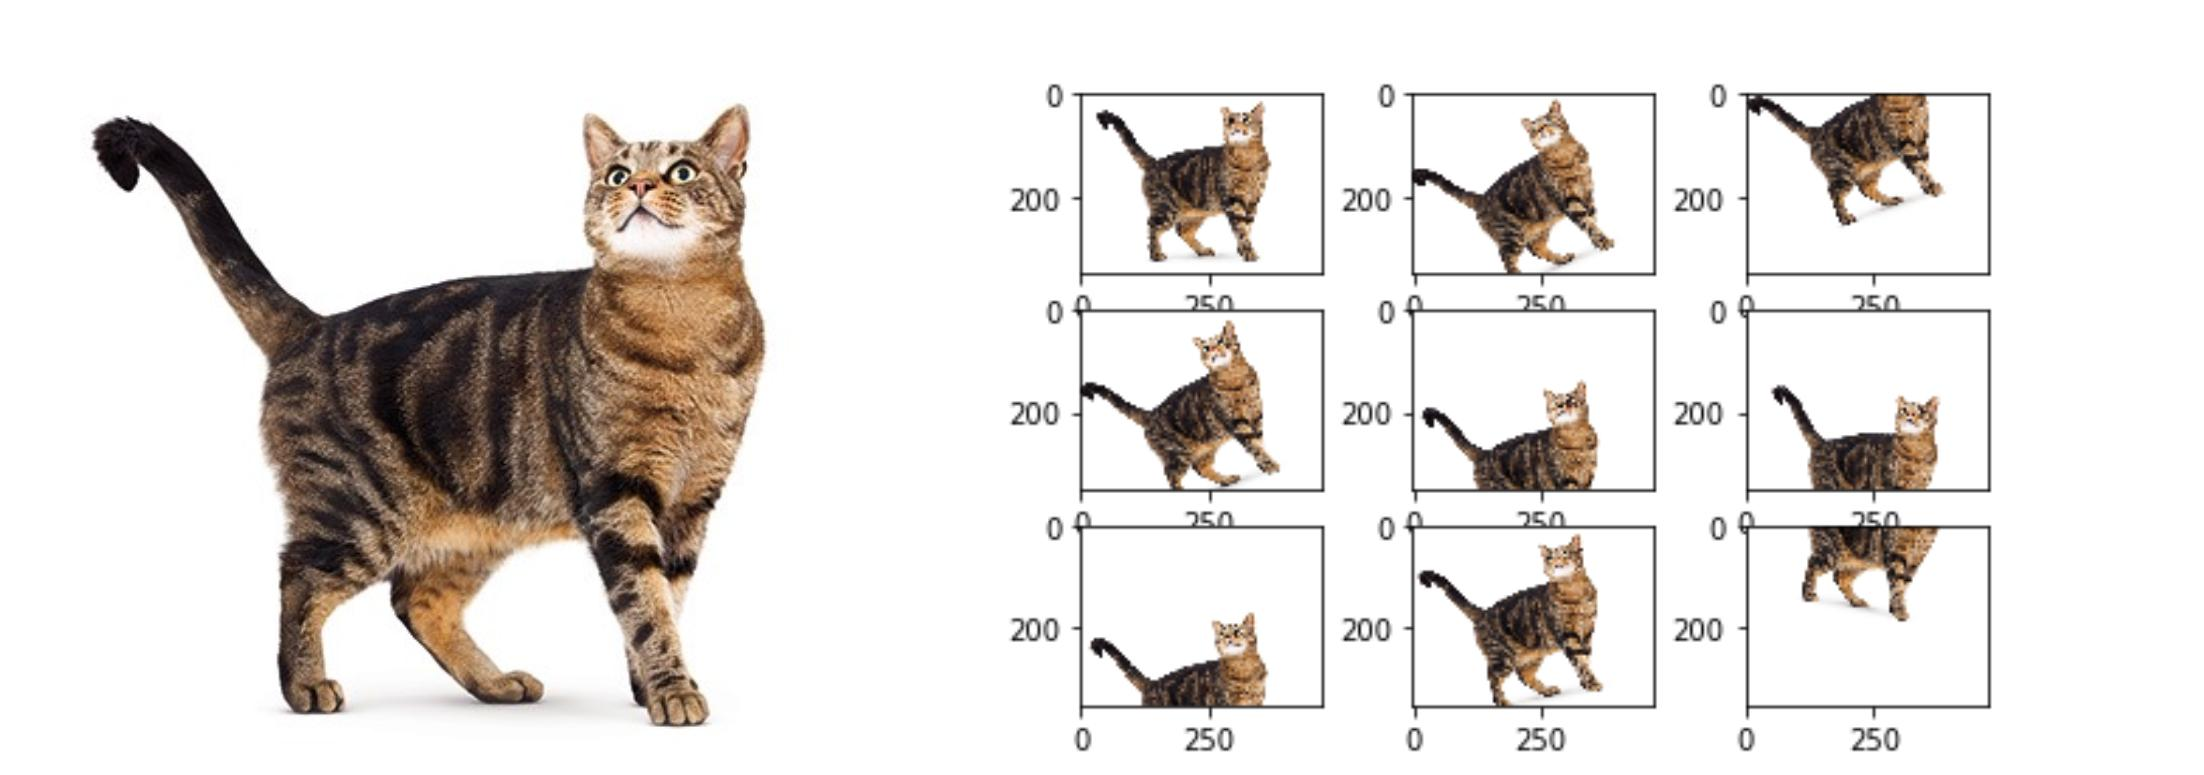
\includegraphics[width=\linewidth]{augmentation}\pause
\end{center}
\begin{PauseHighLight}
  \begin{itemize}
  \item Data augmentation is standard practice in deep learning for
    images\pause{} and makes a very considerable difference\pauseb
  \end{itemize}
\end{PauseHighLight}

\end{slide}

%%%%%%%%%%%%%%%%%%%%%%% Next Slide %%%%%%%%%%%%%%%%%%%%%%%

\begin{slide}
\section{Other Symmetries Exist}

\begin{PauseHighLight}
  \begin{itemize}
    \item In NLP it is now common to translate sentences to a foreign
      language and back to the original language to learn invariance
      to minor changes in the words used\pause
    \item There are cases where we care about sets of objects, but not
      their ordering\pause
    \item An example might be sets of objects in an image or vertices
      in a graph\pause
    \item Here constructing operators that are equivariant (the same
      if we permute the inputs and outputs) can again reduce overfitting\pause
  \end{itemize}
\end{PauseHighLight}

\end{slide}

%%%%%%%%%%%%%%%%%%%%%%% Next Slide %%%%%%%%%%%%%%%%%%%%%%%

\begin{slide}
\section{Normalisation}

\begin{PauseHighLight}
  \begin{itemize}
  \item Sometimes clever normalisation can make a lot of difference to
    the performance of an algorithm\pause
  \item We might do this by feature engineering\pause{} (divide the length on
    the nose by the width between the persons eyes)\pauseb
  \item We might do this by normalising the output\pause---use cosine
    similarity rather than distance
    \begin{align*}
      \cos(\theta) = \frac{\bm{a}^\tr \bm{b}}{\len{\bm{a}}\len{\bm{b}}}\pauseb
    \end{align*}
  \item These make the results invariant\pauseb{} to the distance of
    the camera\pauseb{} or the length of $\bm{a}$ and $\bm{b}$\pauseb
  \end{itemize}
\end{PauseHighLight}

\end{slide}

%%%%%%%%%%%%%%%%%%%%%%% Next Slide %%%%%%%%%%%%%%%%%%%%%%%
\Outline % Group Theory
%%%%%%%%%%%%%%%%%%%%%%% Next Slide %%%%%%%%%%%%%%%%%%%%%%%

\begin{slide}
\section{Group Theory}

\begin{PauseHighLight}
  \begin{itemize}
  \item Symmetries are very well studied in mathematics\pause
  \item The language of symmetries are \emph{groups}\pause
  \item These capture the structure of transformations that represent
    some symmetry\pause
  \item Group theory is highly abstract and it is easy to lose sight
    of its connection to symmetry, but it has proved itself
    extraordinarily powerful in revealing structures\pause
  \end{itemize}
\end{PauseHighLight}

\end{slide}

%%%%%%%%%%%%%%%%%%%%%%% Next Slide %%%%%%%%%%%%%%%%%%%%%%%

\begin{slide}
\section{Groups}

\begin{PauseHighLight}
  \begin{itemize}
  \item Groups consists of a set (we can think of the elements as
    transformations), $\mathcal{G} = \{a,b,\cdots\}$\pause
  \item And an operator ``$\cdot$'' (which we can often think of as
    composition)\pause
  \item That is, $a\cdot b$ we can interpret as apply transformation
    $b$ and then apply transformation $a$\pause
  \item The set and transform form a group if they satisfy four axioms
    \begin{itemize}
    \item closure: for all $a, b \in \mathcal{G}$ then $a\cdot b \in \mathcal{G}$
    \item associativity: $a\cdot (b\cdot c) = (a\cdot b) \cdot c$
    \item existence of an identity $e$ such that $a\cdot e = a$ for
      all $a$
    \item Every element, $a$, has an inverse $a^{-1}$ such that
      $a^{-1}\cdot a = e$\pause
    \end{itemize}
  \end{itemize}
\end{PauseHighLight}

\end{slide} 

%%%%%%%%%%%%%%%%%%%%%%% Next Slide %%%%%%%%%%%%%%%%%%%%%%%

\begin{slide}
\section{Tossing a coin}

\begin{PauseHighLight}
  \begin{itemize}
  \item We consider a coin with two actions
    \begin{itemize}
    \item flip the coin: $f$
    \item leave the coin alone: $e$\pause
    \end{itemize}
  \item These form a group (the cyclic group $C_2$)
    \begin{itemize}
    \item Closure is obvious $f\cdot e =f$, $f\cdot f =e$, $e\cdot e =e$
      and $e \cdot f =f$
    \item Associativity: e.g. $(e\cdot f) \cdot f = e \cdot (f \cdot f)$
    \item $e$ is the identity
    \item $e^{-1}=e$ and $f^{-1}=f$\pause
    \end{itemize}
  \end{itemize}
\end{PauseHighLight}

\end{slide}

%%%%%%%%%%%%%%%%%%%%%%% Next Slide %%%%%%%%%%%%%%%%%%%%%%%

\begin{slide}
\section[-2]{The Four Group}
    
  \pb
  
  \begin{itemize}
  \item A slightly less trivial example represents the set of
    transformations that leaves a rectangle invariant\pauseh
    \vspace*{-0.5cm}
    \begin{center}
      \multipdf[width=0.45\linewidth]{fourGroup}\pause
    \end{center}
    \vspace*{-0.5cm}
  \end{itemize}
  \begin{center} {\small
    \begin{tabular}{c|cccc}
        &e&v&h&r \\ \hline
      e&e&v&h&r \\
      v&v&e&r&h \\
      h&h&r&e&v \\
      r&r&h&v&e 
    \end{tabular}}\pauseb
  \end{center}

\end{slide}


%%%%%%%%%%%%%%%%%%%%%%% Next Slide %%%%%%%%%%%%%%%%%%%%%%%

\begin{slide}
\section[-2]{Non-commutativity}
  
\begin{PauseHighLight}
  \begin{itemize}
  \item Not all groups commute\pause
  \item For 3-d rotations : $R_x \cdot  R_z  \neq R_z\cdot R_x$\pause
  \end{itemize}
\end{PauseHighLight}
\begin{center}
  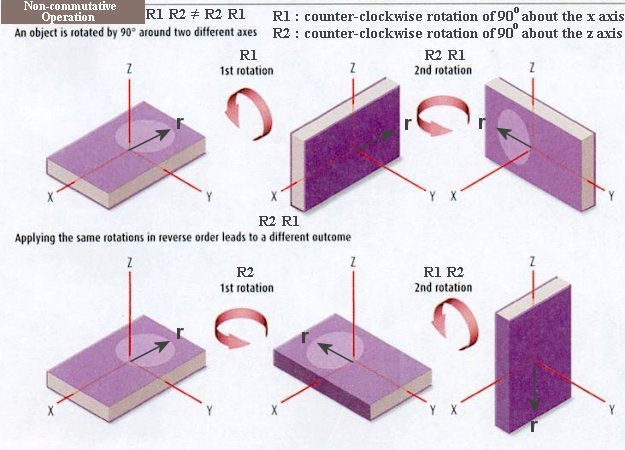
\includegraphics[width=0.7\linewidth]{nonAbelian}\pauseb
\end{center}
\end{slide}

%%%%%%%%%%%%%%%%%%%%%%% Next Slide %%%%%%%%%%%%%%%%%%%%%%%

\begin{slide}
\section[-2]{Associativity}

\begin{PauseHighLight}
  \begin{itemize}
  \item We can think of the elements of a group as transformations
    acting on some object (e.g. rotations of a book)\pause
  \item We consider $\cdot$ to denote composition so $a \cdot b$
    denotes apply action $b$ then action $a$\pause
  \item When we say $c=a \cdot b$ we mean that action $c$ is
    equivalent to apply action $b$ followed by action $a$\pause
  \item Suppose $g = a \cdot b$ and $h = b \cdot c$ then
    \begin{align*}
      g \cdot c &= a \cdot h\pause \\
      (a \cdot b) \cdot c &= a \cdot (b \cdot c)\pause
    \end{align*}
  \item These correspond to an equivalent set of actions\pause
  \end{itemize}
\end{PauseHighLight}


\end{slide}


%%%%%%%%%%%%%%%%%%%%%%% Next Slide %%%%%%%%%%%%%%%%%%%%%%%

\begin{slide}
  \section{Permutations}

\begin{PauseHighLight}
  \begin{itemize}
  \item The set of permutations of $n$ objects form a group (known as
    the symmetric group $S_n$)\pause
  \item The composition of a permutation is a permutation\pause
  \item There is an identity (do nothing)\pause
  \item For every permutation there is an inverse permutation\pause
  \item Obviously $S_n$ has $n!$ elements\pause{} (you can reorder elements in
    n! ways)\pauseb
  \item Permutations have a lot of structure (in terms of elements
    cycling, subgroups, etc.)\pause
  \end{itemize}
\end{PauseHighLight}


\end{slide}

%%%%%%%%%%%%%%%%%%%%%%% Next Slide %%%%%%%%%%%%%%%%%%%%%%%

\begin{slide}
\section{Infinite Groups}

\begin{PauseHighLight}
  \begin{itemize}
  \item The set of integers under addition form a group\pause
  \item Its closed, has an identity, 0, and each element $n$ has an
    inverse $-n$\pause
  \item The group describes the set of discrete shifts\pause
  \item The set of rational number under addition also forms a
    group\pause
  \item Nothing new here, you've known about these since you were a toddler\pauseb
  \end{itemize}
\end{PauseHighLight}

\end{slide}

%%%%%%%%%%%%%%%%%%%%%%% Next Slide %%%%%%%%%%%%%%%%%%%%%%%

\begin{slide}
\section{Continuous Groups}

\begin{PauseHighLight}
  \begin{itemize}
  \item The set of reals under addition form a group and describes
    translations in one dimension\pause
  \item The set of reals excluding 0 form a group under multiplication
    with an identity 1 and inverse of $x$ being $1/x$\pause
  \item These describe scale transformation\pause
  \item These are not terrifically interesting groups\pause{} (or at least
    groups you are so familiar with that they are now boring)\pauseb
  \item Things get more interesting in high dimensional space\pauseb
  \end{itemize}
\end{PauseHighLight}

\end{slide}

%%%%%%%%%%%%%%%%%%%%%%% Next Slide %%%%%%%%%%%%%%%%%%%%%%%

\begin{slide}
\section{Lie Groups}

\begin{PauseHighLight}
  \begin{itemize}
  \item Continuous groups are known as Lie Groups\pause
  \item They describe things like general translational invariance,
    rotational invariance, relativistic invariance\pause
  \item The transformations can be represented by a set of matrices\pause
  \item To study these one looks at infintesimal transformations and
    the algebra between these infintesimal transformations (Lie
    algebras)\pause
  \item This is much studied in physics and occasionally studied in
    machine learning, although more on the sidelines\pause
  \end{itemize}
\end{PauseHighLight}

\end{slide}

%%%%%%%%%%%%%%%%%%%%%%% Next Slide %%%%%%%%%%%%%%%%%%%%%%%

\begin{slide}
  \section{Rotations $SO(n)$}
  
\begin{PauseHighLight}
  \begin{itemize}
  \item The set of $n\times n$ orthogonal matrices (matrices, $\mat{M}$,
    such that $\mat{M}^\tr \mat{M} = \mat{M}\, \mat{M}^\tr = \mat{I}$)
    form a group $O(n)$\pause
  \item Note that $\det(\mat{M}) = \pm 1$\pause
  \item These correspond to rotations and reflections\pause
  \item The group of matrices that don't correspond to reflections
    (where $\det(\mat{M})=1$) form a subgroup $SO(n)$\pause
  \item $SO(2)$ consist of the 2-d rotation matrices
    \begin{align*}
      \begin{pmatrix}
        \cos(\theta) & \sin(\theta) \\
        -\sin(\theta) & \cos(\theta)
      \end{pmatrix}\pause
    \end{align*}
  \end{itemize}
\end{PauseHighLight}

\end{slide}


%%%%%%%%%%%%%%%%%%%%%%% Next Slide %%%%%%%%%%%%%%%%%%%%%%%

\begin{slide}
\section[-2]{Summary}

\begin{PauseHighLight}
  \begin{itemize}
  \item Invariances are important as if a machine properly captures a
    true invariance it can massively limit the space of functions
    being approximated\pause---reducing the chances of finding
    spurious rules\pauseb
  \item Often it is hard to build-in invariances into the machine
    learning model and practitioners will often resort to data
    augmentation in the hope that these invariances can be
    learned\pause
  \item There is a mathematical language around describing the
    structure of symmetries: \emph{group theory}\pause
  \item You should know \textit{group theory} exists, it is occasionally used in machine
    learning, but not that much\pause
  \item I'm not going to expect you to know any details about group
    theory\pauseb
  \end{itemize}
\end{PauseHighLight}

\end{slide}



%%% Local Variables:
%%% TeX-master: "lectures"
%%% End:
